%%%
\usepackage[a4paper, total={6in, 8.6in}]{geometry}
%%
\usepackage{polyglossia}  \setdefaultlanguage{polish}
%%
\usepackage{booktabs}
\usepackage{fontspec}
\setmainfont{Cambria}
\setmathfont{Cambria Math}
%% Supress any other theorems (probably)
\newtheorem{theorem}{}
%%
%% This is not working
%% https://github.com/jgm/pandoc/issues/4384
%%
\AtBeginDocument{%%
 \let\maketitle\relax
  %% Insert title page
 \begin{titlepage}
 \begingroup  
 %% reset
 \setkeys{Gin}{width=210mm,height=300mm}
 \vbox to \textheight{\vss%
   \hbox to\textwidth{\hss
     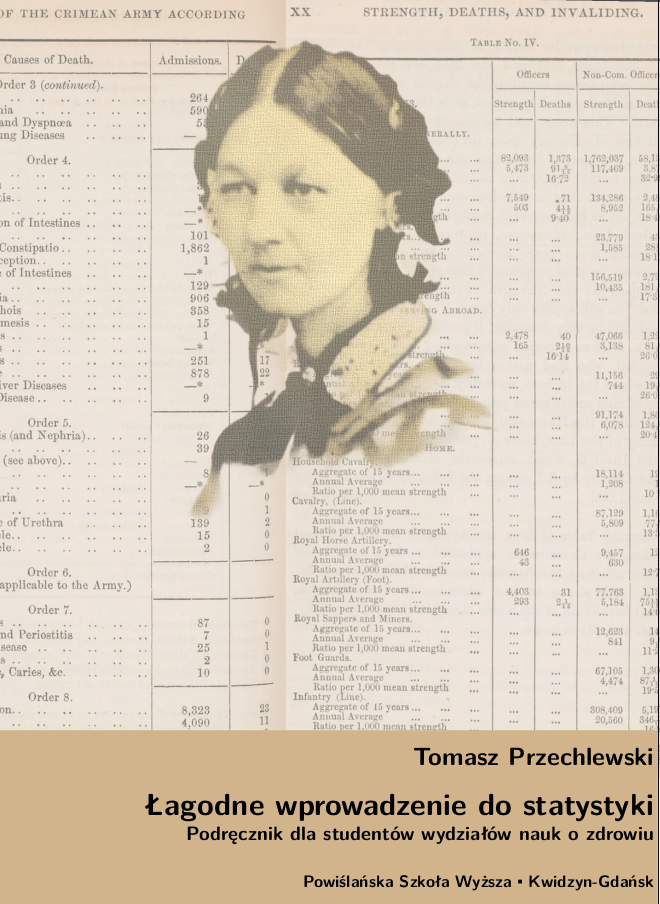
\includegraphics[width=210mm]{Cover_02.png}\hss}
   \vss}
\endgroup
\end{titlepage}
\author{Tomasz Przechlewski\\ Powiślańska Szkoła Wyższa\\(Kwidzyn-Gdańsk)}%
}

\usepackage[most]{tcolorbox}
\newtcolorbox{example}[1][]{%
    colback=black!5,
    colframe=black!5,
    notitle,
    sharp corners,
    enhanced,
    breakable,
}

\font\chineseFont="NotoSansTC-Regular" at 10pt
\def\chinese#1{{\chineseFont #1}}
\edef\bbChar{□}
\edef\bbCharX{☒}
\edef\bbArrowR{→}

\catcode`☒=\active
\catcode`□=\active
\catcode`→=\active
\def☒{\chinese{\bbCharX}} %% bb with X
\def□{\chinese{\bbChar}} %% ballot box
\def→{\chinese{\bbArrowR}} %% right arrow

%%%
